\documentclass[11pt]{article}
\usepackage{authblk}
\usepackage{listings}
\usepackage{xcolor}
\usepackage{graphicx}
\usepackage{float}
\usepackage{hyperref}
\usepackage{indentfirst}

\definecolor{codegreen}{rgb}{0,0.6,0}
\definecolor{codegray}{rgb}{0.5,0.5,0.5}
\definecolor{codepurple}{rgb}{0.58,0,0.82}
\definecolor{backcolour}{rgb}{0.95,0.95,0.92}

\lstdefinestyle{mystyle}{
    backgroundcolor=\color{backcolour},   
    commentstyle=\color{codegreen},
    keywordstyle=\color{magenta},
    numberstyle=\tiny\color{codegray},
    stringstyle=\color{codepurple},
    basicstyle=\ttfamily\footnotesize,
    breakatwhitespace=false,         
    breaklines=true,                 
    captionpos=b,                    
    keepspaces=true,                 
    numbers=left,                    
    numbersep=5pt,                  
    showspaces=false,                
    showstringspaces=false,
    showtabs=false,                  
    tabsize=2
}

\lstset{style=mystyle}

\title{Relazione}
\author{Bruniera Alvise\and Calabrigo Massimo}
\affil{Università degli studi di Udine}
\date{\today}

\begin{document}
\maketitle

\tableofcontents
\section{Introduzione}
Il nostro obiettivo è creare un database postgres, per la gestione di uno studio medico.
Vogliamo registrare informazioni sulle sedute e le terapie dei pazienti, sulle competenze e gli orari di lavoro dei medici, e degli altri dipendenti.
\section{Requisiti e Specifiche}

\subsection{Workflow e fase di specificazione}
Per questo progetto abbiamo deciso di utilizzare un modello iterativo incrementale.
Abbiamo separato il progetto in tre processi: Requisiti e specifiche, Progettazione ed Implementazione;
a loro volta divisi in sottoprocessi:
\begin{enumerate}
    \item Requisiti e Specifiche
    \begin{itemize}
        \item Analisi: lettura del documento, evidenziando punti importanti
        \item Specificazione: riassumere i punti importanti nelle specifiche
        \item Validazione: controllo che le specifiche rispettino il documento, eventualmente tornando all'analisi
    \end{itemize}
    \item Progettazione
    \begin{itemize}
        \item concettuale: stesura e ristrutturazione dell'ER dalle specifiche
        \item logica: traduzione da ER a logico, validazione, ed implementazione su postgres
        \item fisica: scelta degli indici
    \end{itemize}
    \item Implementazione
    \begin{itemize}
        \item Implementazione di operazioni e viste
        \item Analisi statistica dei dati
    \end{itemize}
\end{enumerate}
In questa sezione esponiamo il processo di ``Requisiti e specifiche'', e riportiamo
solo i risultati i risultati finali.

Come prima cosa abbiamo letto il documento con le richieste del cliente (fornito dal professore)
evidenziando concetti principali, annotandoli nel glossario, e richieste importanti. Poi abbiamo iniziato la prima fase di 
analisi dei requisiti, elencando e riordinando quello che avevamo evidenziato.
Prima di passare alla fase di specificazione abbiamo riletto requisiti e documento delle richieste cercando
incompletezze ed errori, quindi abbiamo raffinato i requisiti (seconda iterazione di requisiti).
Quindi siamo passati ad una prima iterazione delle specifiche, in cui abbiamo cominciato a
risolvere le ambiguità, documentando la soluzione nel glossario e semplificando la descrizione.
In una prima fase di validazione abbiamo notato che non erano chiari alcuni dettagli riguardanti
terapie prolungate ed appuntamenti, e se gli appuntamenti fossero da considerarsi sedute programmate;
Quindi siamo tornati all'analisi dei requisiti, risolvendo questo dubbio, ed abbiamo proseguito
con l'ultima fase di specificazione e validazione.

\begin{figure}[H]
    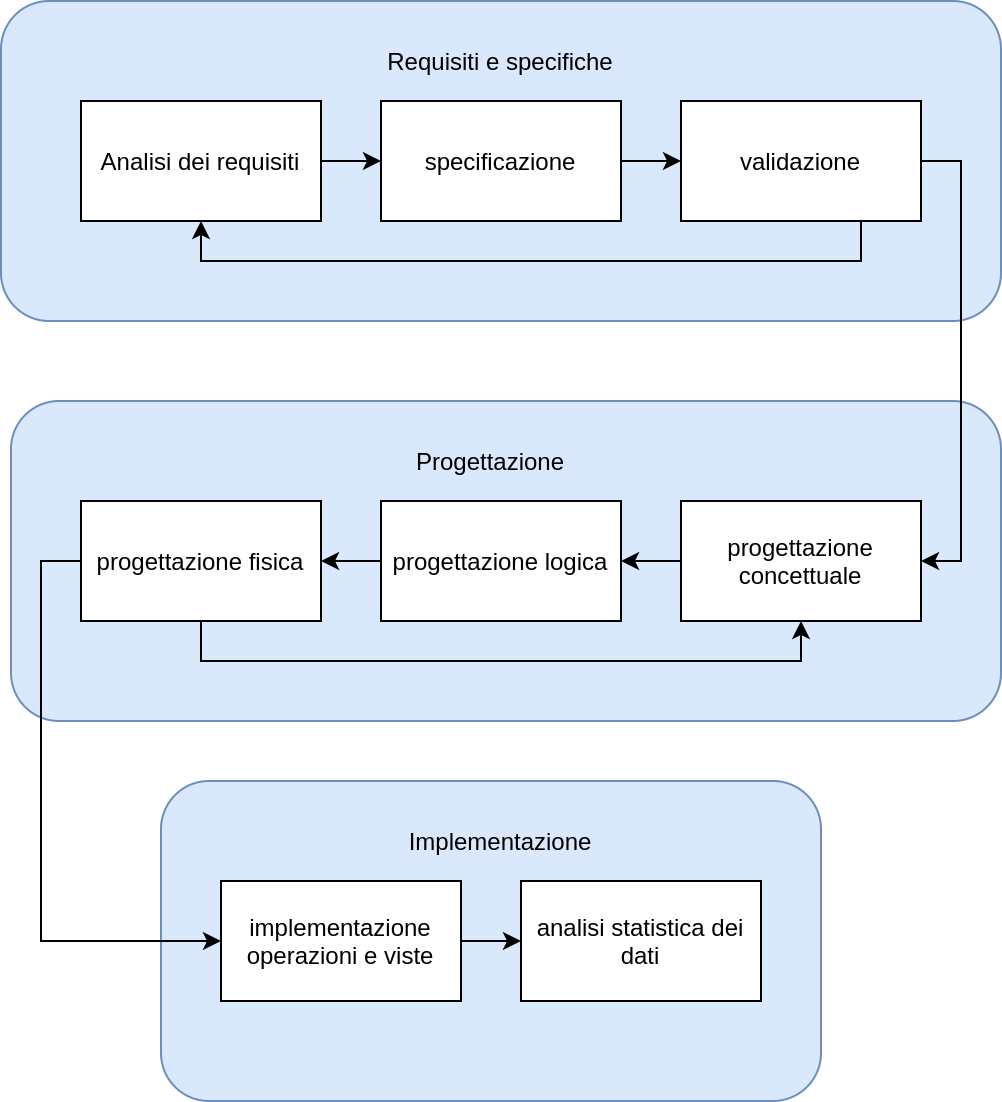
\includegraphics[width=\linewidth]{images/workflow.png}
    \caption{workflow}
    \label{fig:workflow}
\end{figure}
\subsection{Glossario}
Nel corso del processo di specificazione abbiamo annotato i vari termini specifici del
dominio, risolvendo le ambiguità. L'elenco riportato è riferito all'ultima iterazione di
requisiti e specifiche.
\begin{itemize}
\item Medico: Ogni medico può essere interno od esterno.
\item Medico interno: Medico comproprietario dello studio medico.
\item Medico esterno: Medico non comproprietario dello studio medico.
\item Codice-medico: Codice che identifica univocamente un medico.
\item Membro del personale ausiliario: Ogni membro può essere assistente medico, oppure amministrativo, può anche essere entrambe le cose.
\item Codice-personale: Codice che identifica univocamente un membro del personale ausiliario.
\item Paziente: cliente dello studio medico.
\item Paziente regolare: Paziente che si sottopone ad almeno una terapia prolungata.
\item Paziente occasionale: Paziente che si sottopone ad almeno una seduta per un problema urgente.
\item Specializzazione: Titolo di studio acquisito da tutti medici dopo la laurea. (Oculistica, urologia, cardiologia, …)
\item Qualifica: Titoli di studio specifici dei membri del personale ausiliario. (Diploma di ragioneria, laurea in infermieristica, tecnico radiologo, …)
\item Storico: Resoconto periodico.
\item Denominazione: Titolo di un corso di aggiornamento. (“Corso di aggiornamento in pneumologia”, …)
\item Terapia prolungata: Trattamento prolungato a cui si sottopone il paziente.
\item Seduta: Visita occasionale a cui si sottopone il paziente per motivi urgenti. La singola seduta deve risolvere il problema, altrimenti sarebbe parte di una terapia prolungata.
\item Appuntamento: Visita periodica a cui si sottopone il paziente come parte di una terapia prolungata. Quando ci si presenta ad un appuntamento viene comunicato un ambulatorio ed assegnati i membri del personale ausiliario ed i medici che si occuperanno della visita.
\item Appuntamento accettato: appuntamento a cui il paziente si presenta. Può essere terminato o ancora in corso.
\item Appuntamento saltato: appuntamento al quale il paziente non si è presentato.
\item Appuntamento programmato: appuntamento fissato per una data e ora future.
\end{itemize}
\subsection{Requisiti}
Abbiamo riportato requisiti finali, risultato dell'ultima (terza) iterazione di analisi dei requisiti.
Le iterazioni precedenti dei requisiti si trovano nel documento allegato ``Specifiche.docx''
\begin{itemize}
    \item I \emph{medici} possono essere interni od esterni. Un medico è identificato univocamente da un codice-medico, ed ha un nome, un cognome, un indirizzo, un recapito telefonico, ed una o più \emph{specializzazioni}.
    \begin{itemize}
        \item I medici interni sono comproprietari ed hanno diritto su una percentuale degli incassi
        \item I medici esterni hanno una tariffa oraria
    \end{itemize}
    \item Ogni \emph{membro del personale ausiliario} è identificato univocamente da un codice-personale, ed ha un nome, cognome, indirizzo, recapito telefonico (uno), ed una o più qualifiche.
    \begin{itemize}
        \item Gli assistenti medici possono seguire dei corsi di aggiornamento.
        \item Amministrativi.
    \end{itemize}
    \item Ogni \emph{corso di aggiornamento} è identificato univocamente dalla denominazione, dal luogo dove si svolge, dalla data in cui si svolge. Due o più corsi di aggiornamento con la stessa denominazione non possono svolgersi nello stesso luogo alla stessa data.
    \item Ogni mese viene memorizzato \emph{uno storico delle ore lavorative} ordinarie e straordinarie dei medici e dei membri del personale ausiliario.
    \item I \emph{pazienti} possono essere regolari od occasionali. Un paziente è identificato univocamente dal codice fiscale, ed ha un nome, un cognome, un indirizzo, un recapito telefonico, ed una data di nascita.
    \begin{itemize}
        \item I pazienti occasionali si presentano allo studio per un problema urgente da risolvere in una seduta.
        \item I pazienti regolari si sottopongono ad una o più terapie prolungate. Un paziente regolare può essere anche occasionale per un problema urgente estraneo alla terapia prolungata.
    \end{itemize}
    \item Ogni \emph{seduta} è caratterizzata da le persone coinvolte (un paziente, uno o più medici, uno o più membri del personale ausiliario), dalla data, l’ora, e l’ambulatorio in cui si svolge la seduta.
    \item Ogni \emph{terapia prolungata} è caratterizzata dal paziente, da uno specifico tipo di medico e da una data di fine. Una terapia prolungata può essere aperta o chiusa, inizialmente è aperta e quando termina diventa chiusa. Ad un paziente in terapia prolungata aperta possono essere associati uno o più appuntamenti programmati, mentre ad una terapia prolungata chiusa solo appuntamenti accettati o saltati.
    \begin{itemize}
        \item Gli appuntamenti possono essere programmati. In seguito, se il paziente si presenta all’ora e alla data dell’appuntamento programmato, l’appuntamento diventerà accettato, altrimenti diventerà saltato. Degli appuntamenti programmati o saltati non sono noti ambulatorio, medici e membri del personale ausiliario.
    \end{itemize}
    \item Ogni \emph{appuntamento} è caratterizzato dal paziente, dai medici e dai membri del personale ausiliario coinvolti, dalla data, l’ora e l’ambulatorio in cui si svolge.
    \item Lo studio medico dispone di un certo numero di \emph{ambulatori}, dove ogni ambulatorio è identificato univocamente da una lettera.
\end{itemize}
\subsection{Specifiche}
Come per i requisiti, abbiamo riportato solo l'ultima iterazione (seconda) delle specifiche.
Sullo stesso file (``Specifiche.docx'') si trova anche la prima iterazione.
\begin{itemize}
    \item Il medico è identificato univocamente dal codice-medico ed è caratterizzato da nome, cognome, indirizzo, un unico recapito telefonico e una o più specializzazioni. I medici interni hanno diritto a una percentuale degli incassi e i medici esterni hanno una tariffa oraria. Un medico si occupa di zero o più appuntamenti accettati. Il medico si occupa di zero o più sedute.
    \item Un medico ha una o più specializzazioni.
    \item Le specializzazioni sono: Oculistica, urologia, pneumologia, …
    \item Il membro del personale ausiliario è identificato univocamente da codice-personale ed è caratterizzato da nome, cognome, indirizzo, da un unico recapito telefonico e da una o più qualifiche. Il membro del personale ausiliario può essere amministrativo, assistente medico, od entrambi. Il membro del personale ausiliario partecipa a zero o più appuntamenti accettati.
    \item Gli assistenti medici possono seguire nessuno o più corsi di aggiornamento.
    \item Le qualifiche sono: Diploma di ragioneria, laurea in infermieristica, tecnico radiologo, …
    \item Un corso di aggiornamento è identificato univocamente dalla denominazione, dal luogo e data in cui si svolge.
    \item Lo storico mantiene per ogni mese il numero di ore ordinarie e straordinarie dei medici e dei membri del personale ausiliario.
    \item Il paziente è identificato univocamente dal codice fiscale, ed è caratterizzato da nome, cognome, indirizzo, un unico recapito telefonico e dalla data di nascita. Il paziente è occasionale, regolare o entrambi. Il paziente regolare si sottopone ad una o più terapie prolungate aperte, mentre il paziente occasionale si sottopone ad una o più sedute. Il paziente è sia regolare che occasionale se ha almeno una terapia prolungata aperta e si sottopone a una seduta.
    \item Ogni seduta è caratterizzata dal paziente, da uno o più medici, da uno o più membri del personale ausiliario, dalla data, dall’ora, e dall’ambulatorio in cui si svolge la seduta.
    \item Ogni terapia prolungata è caratterizzata dal paziente, da uno specifico tipo di medico da una data di inizio; e da una data di fine (quest’ultima è inserita alla fine della terapia prolungata). Una terapia prolungata può essere aperta o chiusa, inizialmente è aperta e quando termina diventa chiusa. Ad un paziente in terapia prolungata aperta possono essere associati uno o più appuntamenti programmati, tra cui almeno uno programmato.
    \item Ad una terapia prolungata chiusa possono essere associati appuntamenti accettati o appuntamenti saltati.
    \item Ogni appuntamento è caratterizzato dalla terapia prolungata, dalla data, l’ora e l’ambulatorio in cui si svolge. Un appuntamento può essere programmato, accettato o saltato.
    \begin{itemize}
        \item È programmato quando è fissato per una data e ora future.
        \item È accettato quando la data e l’ora sono passate, e il paziente si è presentato, e gli vengono assegnati uno o più medici e uno o più membri del personale ausiliario
        \item È saltato accettato quando la data e l’ora sono passate, e il paziente non si è presentato
    \end{itemize} 
    \item Lo studio medico dispone di un certo numero di ambulatori, dove ogni ambulatorio è identificato univocamente da una lettera.
    \item Quando si assegna un medico a un appuntamento tra le specializzazioni del medico ci deve essere quella del tipo di specializzazione di terapia.

\end{itemize}

\subsection{Diagramma dei Casi d'Uso}

Per facilitare la progettazione abbiamo anche abbozzato un diagramma dei casi d'uso, che rappresenta alcune operazioni comuni che ci aspettiamo dal sistema gestito da questa base di dati.

\begin{figure}[H]
    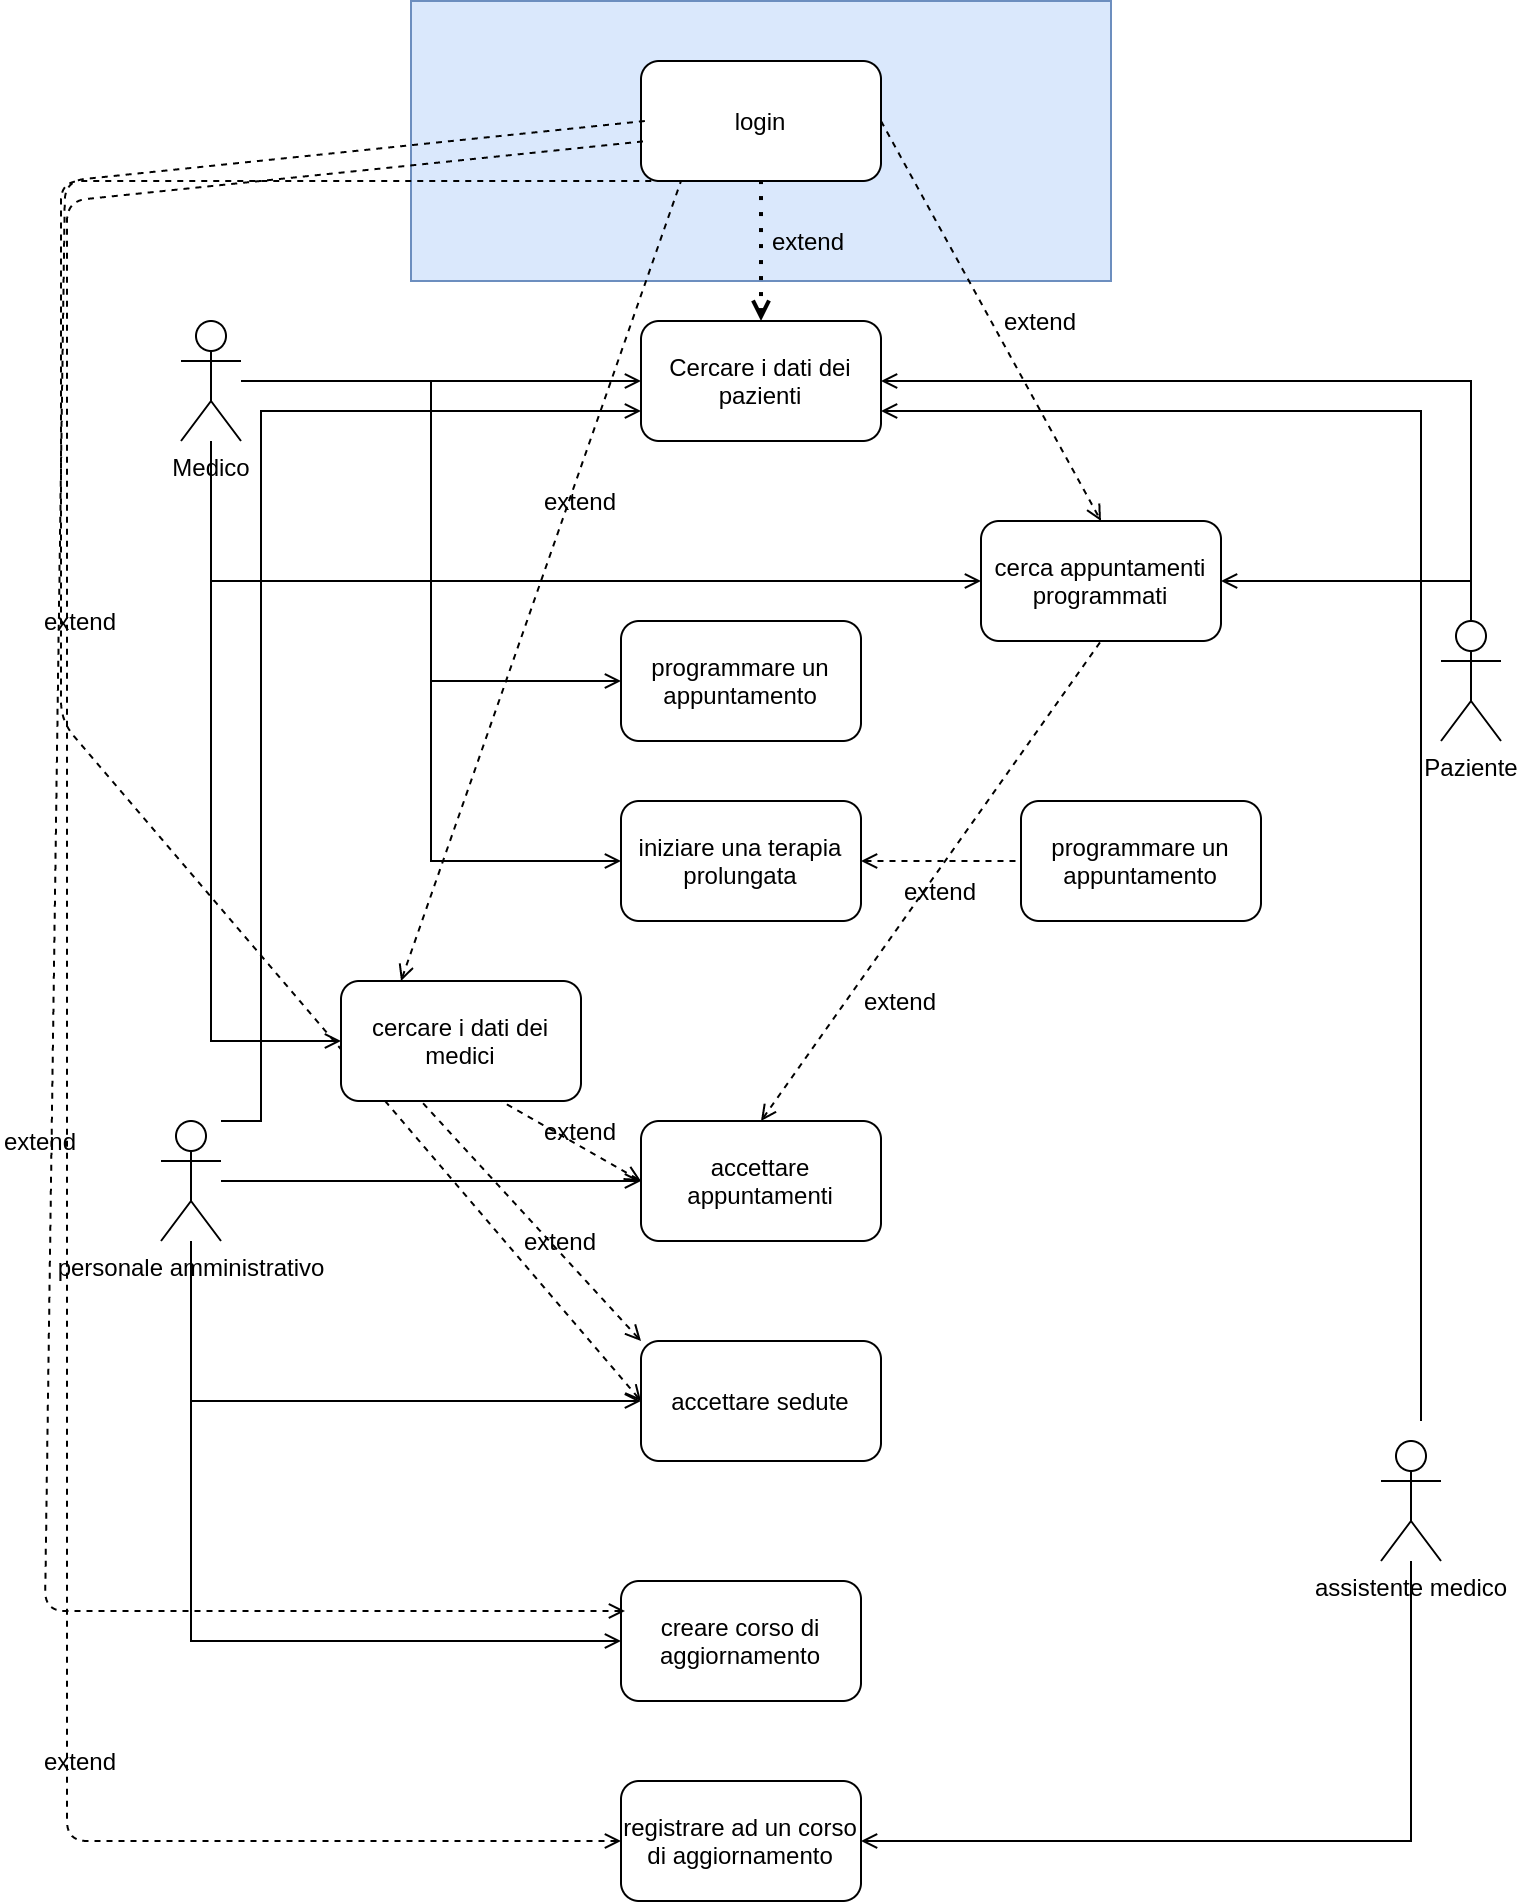
\includegraphics[width=\linewidth]{images/UseCases.png}
    \caption{Casi d'Uso}
    \label{fig:usecases}
\end{figure}

\section{ER e relazionale}

\subsection{ER}
\begin{figure}[H]
    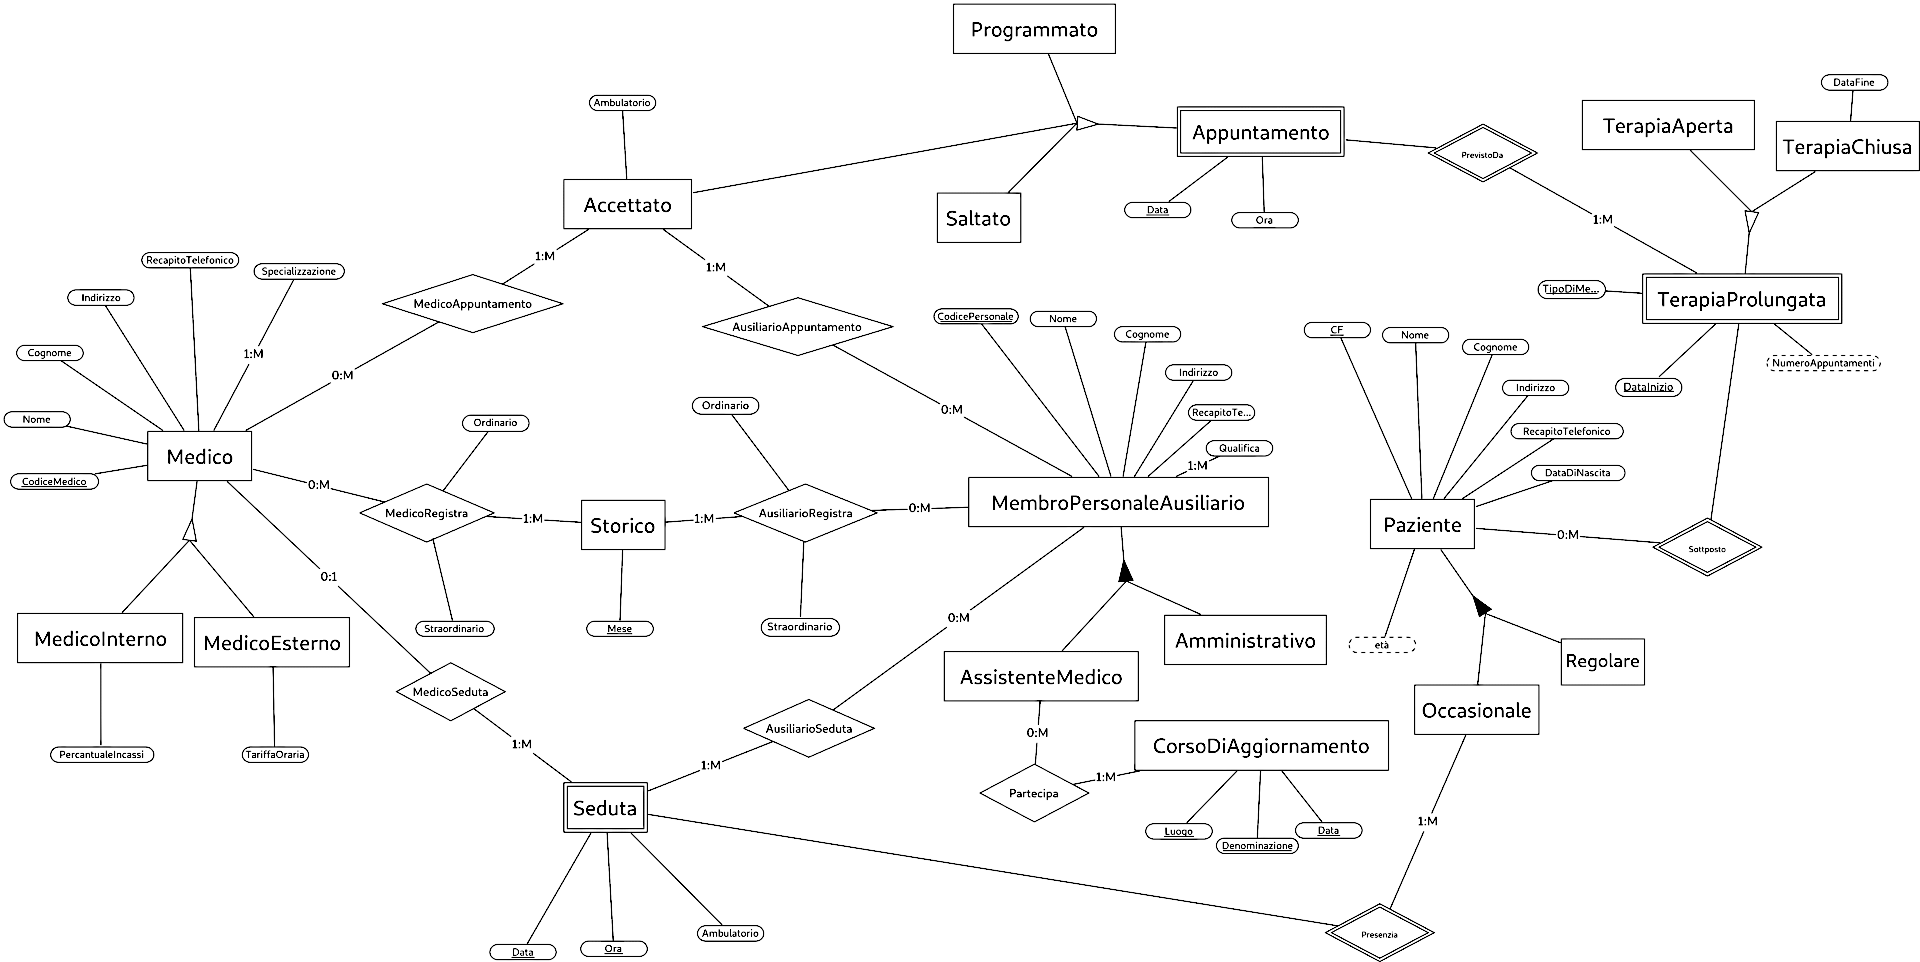
\includegraphics[width=\linewidth]{images/ER1.png}
    \caption{ER}
    \label{fig:ER}
\end{figure}

\subsubsection{Stesura}
Per la stesura dell'ER abbiamo seguito un approccio misto di progettazione.
Inizialmente abbiamo associato ad ogni punto delle specifiche, una entità, tranne che In
alcuni casi particolari in cui un'entità era descritta da più punti (esempio: i primi tre punti
descrivono due entità). Quindi ci siamo divisi le entità tra i membri del gruppo, ed 
individualmente le abbiamo raffinate e messe in relazione tra di loro.

Finito il lavoro individuale, abbiamo aggregato quanto prodotto individualmente in un unico ER 
aggiungendo le relazioni tra le due parti, e raffinato ulteriormente le entità, in particolare
i collegamenti tra le parti sviluppate individualmente. Abbiamo poi verificato, che l'ER rispettasse le specifiche,
anche analizzando i cicli; ad esempio consideriamo il ciclo: Specializzazioni - terapia prolungata - appuntamento accettato 
- Medico - Specializzazioni, detto che ad ogni terapia prolungata è associata una specializzazione, ed ogni medico può avere più
specializzazioni (od anche nessuna), il medico che si occupa di un appuntamento, associato ad una terapia, deve essere specializzato
\emph{almeno} nella stessa specializzazione associata alla terapia. Molti cicli non erano problematici,
quelli che lo erano sono stati risolti con un trigger \ref{trig:trigger1}.
\subsubsection{Ristrutturazione}
\begin{figure}[H]
    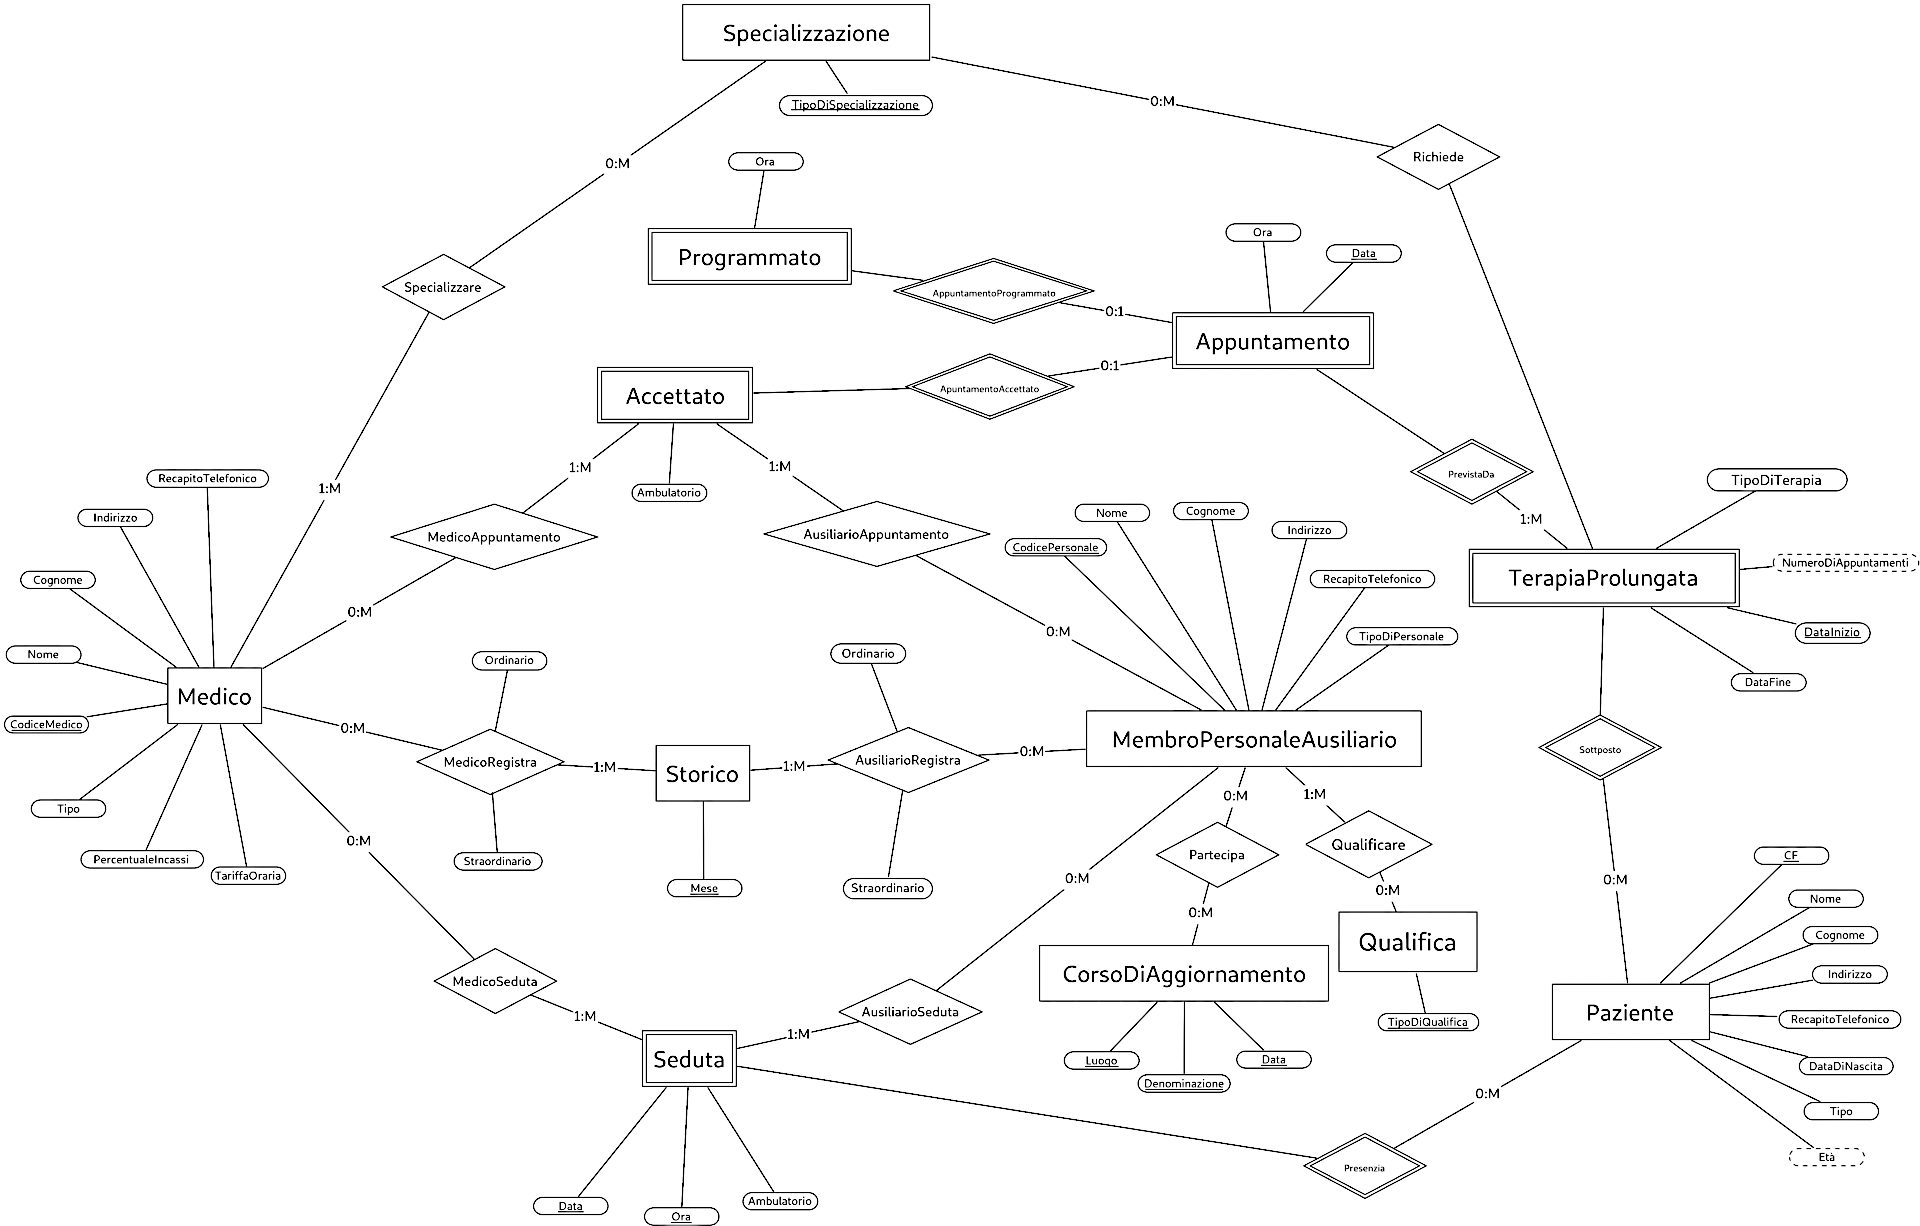
\includegraphics[width=\linewidth]{images/ER_Ristrutturato2.png}
    \caption{ER Ristrutturato}
    \label{fig:ER_Ristrutturato}
\end{figure}
In questa fase abbiamo risolto le specializzazioni, gli attributi composti, ed altri costrutti non rappresentabili direttamente in relazionale (come gli attributi con cardinalità multipla). A contario della fase di stesura, la fase di ristrutturazione è stata svolta direttamente in coppia, invece che separando i compiti, questo sia per poter decidere meglio la soluzione più adatta quando un costrutto poteva essere risolto in più modi diversi, che per permettere a tutto il gruppo di prendere ``familiarità'' anche con le parti dello schema ER di cui non si è occupato personalmente.
Come per i sottoprocessi precedenti, dopo la prima fase di ristrutturazione è seguita una fase di validazione, in cui abbiamo riesaminato l'intero schema, per controllare che fosse adeguato; quindi, insoddisfatti di come era stata trasformata la generalizzazione dell'entità ``Appuntamento'', abbiamo corretto l'errore in una seconda iterazione, prima di dichiarare conclusa la ristrutturazione.

All'atto pratico, abbiamo deciso di non reificare ne la specializzazione di ``Medico'' (in MedicoInterno e MedicoEsterno), ne la specializzazione di ``MembroPersonaleAusiliario'' (in AssistenteMedico ed Amministrativo), ma di inserire degli attributi ``Tipo'' e ``TipoDiPersonale'' per indicare la a quale entità specializzata appartengono, oltre all'aggiunta di opportuni vincoli e trigger. Lo stesso è stato fatto per l'entità ``Paziente''.
La specializzazione dell'entità ``Appuntamento'', invece, era stata inizialmente reificata completamente nelle sue tre varianti specializzate (Programmato, Accettato, e Saltato); ma nella seconda iterazione di ristrutturazione è stata rimossa l'entità ``Saltato'' perché ridontante, in quanto era sufficiente controllare la data e l'ora prefissate per l'appuntamento, e l'appartenenza o meno all'entità ``Accettato'' per sapere se un appuntamento era programmato o saltato. L'entità ``Programmato'' è stata mantenuta, nonostante fosse superflua come ``Saltato'' in seguito all'analisi delle ridondanze \ref{er:ridondanze1}. Inoltre, si è scelto di reificare ``Specializzazione'' per semplificare altre operazioni sulla base di dati, principalmente per garantire il vincolo che richiede che il medico associato ad un'appuntamento possieda la specializzazione richiesta dalla terapia.

\subsubsection{Analisi delle ridondanze}
\label{er:ridondanze1}
\begin{table}[H]
\begin{tabular}{|c|c|c|}
\hline \textbf{Nome}             & \textbf{Tipo} & \textbf{\#istanze} \\
\hline Medico                    & E             & 20                 \\
\hline Specializzazione          & E             & 20                 \\
\hline Programmato               & E             & 500                \\
\hline Accettato                 & E             & 20000              \\
\hline Storico                   & E             & 120                \\
\hline Seduta                    & E             & 300000             \\
\hline Saltato                   & E             & 100                \\
\hline Appuntamento              & E             & 20600              \\
\hline MembroPersonaleAusiliario & E             & 50                 \\
\hline CorsoDiAggiornamento      & E             & 50                 \\
\hline Qualifica                 & E             & 20                 \\
\hline TerapiaProlungata         & E             & 7000               \\
\hline Paziente                  & E             & 6000               \\
\hline Specializzare             & R             & 30                 \\
\hline MedicoAppuntamento        & R             & 25000              \\
\hline MedicoRegistra            & R             & 2400               \\
\hline MedicoSeduta              & R             & 301000             \\
\hline ApppuntamentoSaltato      & R             & 100                \\
\hline AppuntamentoProgrammato   & R             & 500                \\
\hline AppuntamentoAccettato     & R             & 20000              \\
\hline AusiliarioAppuntamento    & R             & 20000              \\
\hline AusiliarioRegistra        & R             & 6000               \\
\hline AusiliarioSeduta          & R             & 20000              \\
\hline Richiede                  & R             & 7000               \\
\hline PrevistaDa                & R             & 20600              \\
\hline Partecipa                 & R             & 500                \\
\hline Qualificare               & R             & 70                 \\
\hline Presenzia                 & R             & 300000             \\
\hline Sottoposto                & R             & 7000               \\
\hline
\end{tabular}
    \caption{Numero di istanze di entità e relazioni}
    \label{tab:istanze}
\end{table}

\begin{table}[H]
\begin{tabular}{|c|c|c|}
\hline \textbf{Operazioni}                      & \textbf{Tipo} & \textbf{Frequenza} \\
\hline Cercare dati pazienti                    & Interattivo   & 60                 \\
\hline Cercare appuntamenti programmati         & Interattivo   & 120                \\
\hline Programmare un appuntamento              & Interattivo   & 60                 \\
\hline Accettare un appuntamento                & Interattivo   & 60                 \\
\hline Accettare sedute                         & Interattivo   & 100                \\
\hline Creare corso di aggiornamento            & Interattivo   & 0.1                \\
\hline Registrarsi ad un corso di aggiornamento & Interattivo   & 0.1                \\
\hline Cercare dati dei medici                  & Interattivo   & 200                \\
\hline Iniziare una terapia prolungata          & Interattivo   & 2                  \\
\hline Segna appuntamenti saltati               & Interattivo   & 1                  \\
\hline
\end{tabular}
    \caption{Frequenza e tipo delle operazioni}
    \label{tab:operazioni}
\end{table}

\begin{table}[H]
\begin{tabular}{|c|c|c|c|}
\hline \textbf{Cercare appuntamenti programmati} & \textbf{Con}   & \textbf{60000}   &               \\
\hline \textbf{Concetto}                         & \textbf{Tipo}  & \textbf{Accesso} & \textbf{Tipo} \\
\hline Programmato                               & E              & 500              & R             \\
\hline \textbf{Cercare appuntamenti programmati} & \textbf{Senza} & 2472000          &               \\
\hline \textbf{Concetto}                         & \textbf{Tipo}  & \textbf{Accesso} & \textbf{Tipo} \\
\hline Appuntamento                              & E              & 20600            & R             \\
\hline
\end{tabular}
    \caption{Analisi appuntamenti programmati}
    \label{tab:programmati}
\end{table}

\begin{table}[H]
\begin{tabular}{|c|c|c|c|}
\hline \textbf{Segna appuntamenti saltati} & \textbf{Con}   & \textbf{504}     &               \\
\hline \textbf{Concetto}                   & \textbf{Tipo}  & \textbf{Accesso} & \textbf{Tipo} \\
\hline Saltato                             & E              & 1                & W             \\
\hline Programmato                         & E              & 500              & R             \\
\hline Programmato                         & E              & 1                & W             \\
\hline \textbf{Segna appuntamenti saltati} & \textbf{Senza} & 502              &               \\
\hline \textbf{Concetto}                   & \textbf{Tipo}  & \textbf{Accesso} & \textbf{Tipo} \\
\hline Programmato                         & E              & 500              & R             \\
\hline Programmato                         & E              & 1                & W             \\
\hline
\end{tabular}
    \caption{Analisi appuntamenti saltati}
    \label{tab:saltati}
\end{table}

Per l'anilisi delle ridondanze abbiamo cominciato elencando la quantità di istanze di ogni entità e relazione dello schema \ref{tab:istanze}, cercando di utilizzare numeri adeguati ad uno studio moderatamente grande (20 medici) e già in attività da qualche anno (almeno una decina); nella fase di popolazione \ref{pop:popolazione} abbiamo cercato, dove possibile, di tenere in considerazione la quantità di istanze prevista in questa fase, per mantenere la validità dell'analisi.

Successivamente abbiamo trovato la frequenza delle operazioni prese dal diagramma dei casi d'uso \ref{fig:usecases}, tenendo in considerazione anche il numero di istanze (ad esempio, più appuntamenti programmati vuol dire più accettazioni) previsto in precedenza. A questo punto ne abbiamo scelto alcune (ne sono state riportate due: \ref{tab:programmati} \ref{tab:saltati}) di queste operazioni legate a delle ridondanze dello schema, e abbiamo calcolato come cambiava il numero di accessi giornalieri alla base di dati con e senza le ridondanze. Ne è risultato che mantenere l'entità ridondante ``Programmato'' portava ad una notevole riduzione degli accessi alla base di dati, quindi si è deciso di mantenere l'entità; mantenere l'entità ``saltato'', invece, comportava una riduzione minima, quinsi si è scelto di rimuovere la ridondanza.

\subsection{Relazionale}
Una volta ristrutturato, l'ER è pronto per essere tradotto in relazionale, e quindi le entità e le relazioni dell'ER, fanno posto alle relazioni del relazionale, e subito dopo abbiamo 
validato la nuova struttura, verificando che il relazionale appena prodotto rispettasse le forme normali.
\subsubsection{Traduzione}

Per prima cosa abbiamo iniziato identificando le entità principali dell'ER che si sarebbero trasformate in singole relazioni, e che avevamo già identificato nella fase di ristrutturazione come medico, membroPersonaleAusiliario, paziente, terapiaProlungata, ...

Poi ci siamo concentrati sulle relazioni molti a molti (dell'ER), per trasformarle in relazioni (in relazionale), anche queste erano già state identificate nella fase precedente di ristrutturazione; relazioni come: AusiliarioSeduta, MedicoRegistra, Specializzare, ...

Una volta ottenute le relazioni (del relazionale), abbiamo assegnato i vincoli di chiave primaria, secondo i campi di chiave primaria dell'ER, e le chiavi esterne, facendo attenzione a porle nelle relazioni (del relazionale) ottenute da relazioni molti a molti (dell'ER).

\begin{itemize}
    \item Medico(\underline{codice medico}, recapito telefonico, indirizzo, cognome, nome, tipo, percentuale incassi (nullable), tariffa oraria (nullable))
    \item Seduta(\underline{data, ora, cf (ext)}, ambulatorio)
    \item MedicoSeduta(\underline{codice medico(ext), data(ext), ora(ext), cf (ext)})
    \item AusiliarioSeduta(\underline{codice personale(ext), data(ext), ora(ext), cf (ext)})
    \item MembroPersonaleAusiliario(\underline{codice personale}, nome, cognome, indirizzo, recapito telefonico, tipoDiPersonale)
    \item Storico(\underline{mese})
    \item AusiliarioRegistra(\underline{mese (ext), codice personale (ext)}, ordinario, straordinario)
    \item MedicoRegistra(\underline{mese (ext), codice medico (ext)}, ordinario, straordinario)
    \item CorsoDiAggiornamento(\underline{Luogo, denominazione, data})
    \item Partecipa(\underline{CodicePersonale, luogo, denominazione, data (ext)})
    \item Qualifica(\underline{TipoDiQualifica})
    \item Qualificare(\underline{codicePersonale, tipoDiQualifica (ext)})
    \item Specializzazione(\underline{tipoDiSpecializzazione})
    \item Specializzare(\underline{CodiceMedico(ext), tipoDiSpecializzazione (ext)})
    \item Paziente(\underline{Cf}, nome, cognome, indirizzo, recapito telefonico, data di nascita, tipo, età)
    \item TerapiaProlungata(\underline{DataDiInizio, cf (ext)}, dataDiFine (nullable), tipoDiTerapia, tipoDiSpecializzazione (ext), numeroAppuntamento)
    \item Appuntamento(\underline{data, DataDiInizio (ext), CF (ext)}, ora) [unique: (data, ora, CF)]
    \item Programmato(\underline{data (ext), DataDiInizio (ext), CF (ext)}, ora)
    \item Accettato(\underline{data(ext), DataDiInizio (ext), CF (ext)}, ambulatorio)
    \item MedicoAppuntamento(\underline{codiceMedico, data, DataDiInizio (ext), CF (ext)})
    \item AusiliarioAppuntamento(\underline{codicePersonale, data, DataDiInizio (ext), CF (ext)})
\end{itemize}

\subsubsection{Validazione e forme normali}
\textbf{Prima forma normale}: Lo schema relazionale rispetta la prima forma normale sono stati eliminati in fase di ristrutturazione gli attributi multivalore, 
e di conseguenza non esistono campi di riga i e colonna j di nessuna delle istanze delle relazioni dello schema che abbiano più di un valore.\\

\textbf{Seconda forma normale}: Tutti gli attributi non chiave dipendono (direttamente o tramite catene di dipendenze), dalla chiave primaria completa per ogni relazione, qui scriviamo le più articolate:

\begin{itemize}
    \item Medico: tariffa oraria e percentuale incassi non dipendono da tipo perché per uno stesso tipo di medico, possono esserci diverse percentuali o tariffe orarie, mentre per uno stesso codice medico, ci sono le stesse percentuali incassi e tariffa oraria.
    \begin{itemize}
        \item codice medico $\rightarrow$ recapito telefonico
        \item codice medico $\rightarrow$ indirizzo
        \item codice medico $\rightarrow$ nome
        \item codice medico $\rightarrow$ cognome
        \item codice medico $\rightarrow$ tipo
        \item codice medico $\rightarrow$ percentuale incassi
        \item codice medico $\rightarrow$ tariffa oraria
    \end{itemize}

    \item Seduta:
    \begin{itemize}
        \item Cf $\rightarrow$ data
        \item Cf $\rightarrow$ ora
        \item Cf $\rightarrow$ ambulatorio
    \end{itemize}
    \item MembroPersonaleAusiliario:
    \begin{itemize}
        \item Codice medico $\rightarrow$ nome
        \item Codice medico $\rightarrow$ cognome
        \item Codice medico $\rightarrow$ indirizzo
        \item Codice medico $\rightarrow$ recapito telefonico
        \item Codice medico $\rightarrow$ tipo di personale
    \end{itemize}

    \item AusiliarioRegistra:
    \begin{itemize}
        \item Mese, codice personale $\rightarrow$ ordinario
        \item Mese, codice personale $\rightarrow$ straordinario
    \end{itemize}

    \item Paziente:
    \begin{itemize}
        \item Cf $\rightarrow$ nome
        \item Cf $\rightarrow$ cognome
        \item Cf $\rightarrow$ indirizzo
        \item Cf $\rightarrow$ recapito telefonico
        \item Cf $\rightarrow$ data di nascita
        \item Cf $\rightarrow$ tipo
        \item Cf $\rightarrow$ età
    \end{itemize}

    \item TerapiaProlungata:
    \begin{itemize}
        \item Data di Inizio, cf $\rightarrow$ data di fine
        \item Data di Inizio, cf $\rightarrow$ tipo di terapia
        \item Data di Inizio, cf $\rightarrow$ tipo di specializzazione
        \item Data di Inizio, cf $\rightarrow$ numero appuntamenti
    \end{itemize}
\end{itemize}

In realtà è facile vedere che non ci sono catene di dipendenze, quindi le relazioni saranno anche in terza forma normale.\\

\textbf{Terza forma normale}: Dall’analisi effettuata è risultato che ogni attributo non chiave dipende direttamente dalla chiave composta, 
e che non esistono dipendenze transitive, quindi tutte le relazioni analizzate sono in terza forma normale.\\
\\
Visto che il relazionale rispetta le forme normali, lo riteniamo validato e possiamo passare alla fase successiva di creazione degli indici.


\section{Progettazione fisica}
\subsection{Scelta degli indici}
indici.sql


\section{Alcuni Trigger e Query}
\subsection{Trigger}
\label{trig:trigger1}
trigger.sql, codice + spiega il trigger
\subsection{query}
interrogazioni.sql, codice + spiega la query
\begin{lstlisting}[language=SQL]
    -- tutti i medici che hanno visitato il paziente ABCDEF
    select codiceMedico, nome, cognome
    from medico m
    where codiceMedico = any (select codiceMedico
        from medicoSeduta
        where cf = 'ABCDEF')
    or codiceMedico = any (select codiceMedico
        from medicoAppuntamento
        where cf = 'ABCDEF');
\end{lstlisting}


\section{Popolazione ed analisi}
\subsection{Popolazione}
\label{pop:popolazione}
Per avere dei dati su cui eseguire l'analisi, quindi provare quesy ed il comportamento dei vari vincoli e trigger, abbiamo popolato in modo casuale il database utilizzando uno script in R, che si collega al database e, partendo da dei campioni (elenchi casuali di nomi, cognomi, indirizzi, date, etc. recuperati da Internet) genera dei dati casuali da memorizzare sulla base di dati.
Per maggiore coerenza con il resto del progetto, abbiamo scelto il numero di righe genarate, tenendo conto del numero di istanze ipotizzato per l'analisi delle ridondanze \ref{tab:istanze}, ma (escluse alcune tabelle come ``Accettato'', il cui numero di righe è casuale) generalmente generandone una quantità maggiore.

Il lavoro si è svolto in due fasi ed anche questa volta è stato diviso tra i membri del gruppo. Nella prima fase abbiamo separato le tabelle corrispondenti alle entità dell'ER, queste tabelle sono state suddivise in due gruppi di simili dimensioni di cui ciascun membro si è occupato individualmente producendo uno script; ci siamo poi incontrati per mettere insieme i due script in uno unico che popolasse tutte le entità.
Nella seconda fase abbiamo gestito allo stesso modo le tabelle che rappresentavano le relazioni dell'ER, eventualmente leggendo dal database dati scritti dagli script della prima fase per assicurarsi di rispettare alcuni vincoli di integrità.

Lo script è stato scritto in modo da generare dati che rispettassero i vincoli implementati nella base di dati, questo anche a discapito dell'efficienza, sapendo che anche così i dati vengono generati in pochi secondi ed è sufficiente farlo una volta sola.
Tuttavia a volte può generare delle chiavi ripetute per le tabelle ``Seduta'' e ``TerapiaProlungata''; nonostante la quantità di dati generati, questo evento si verifica poco spesso, ed in quel caso è sufficiente cancellare i dati già scritti e riprovare. Visto che si trattava (considetata la frequenza del problema, e l'utilizzo di un tale script) di un problema marginale, abbiamo deciso di non risolverlo ma sottolinearne semplicemente la possibilità.

\subsubsection{Snippets}
Riportiamo alcuni snippets interessanti del codice che genera i dati di popolazione, il codice completo dello script è disponibile nel file ``popolazione.r''.\\

\textbf{Generazione sedute}
\begin{lstlisting}[language=R]
## Omessa la generazione di cf (contenente i codici fiscali di tutti i pazienti) e cf_terapia (contenente i codici dei pazienti in terapia prolungata)

# Seduta
# Questo campionamento e' la causa delle eventuali chiavi ripetute
cf_seduta <- sample(cf, 20000, replace=T)
ora <- sample(1:24, 20000, replace=T)
ambulatorio <- sample(LETTERS[1:26], 20000, replace=T)
data_seduta <- sample(dat, 20000, replace=T)

# Controllo che tutti i pazienti siano regolari od occasionali, e memorizzo l'informazione su un array
tipo = c()
for(i in 1:length(cf)) {
    regolare <- cf[i]%in%cf_terapia
    occasionale <- cf[i]%in%cf_seduta
    if(regolare && occasionale) {
        tipo[i] <- "entrambi"
    } else {
        if(regolare) {
            tipo[i] <- "regolare"
        } else {
            if(occasionale) {
                tipo[i] <- "occasionale"
            } else {
                # Se il paziente non e' ancora ne regolare ne occasionale, aggiungo una seduta rendendolo occasionale
                tipo[i] <- "occasionale"
                append(cf_seduta, cf[i])
                append(ora, sample(1:24, 1, replace=T))
                append(ambulatorio, sample(LETTERS[1:26], 1, replace=T))
                append(data_seduta, sample(dat, 1, replace=T))
            }
        }
    }
}
\end{lstlisting}

\textbf{Generazione terapie prolungate}
\begin{lstlisting}[language=R]
# Terapie aperte (frame di appoggio per controllare i vincoli)
aperte <- data.frame(matrix(ncol = 2, nrow=0))
colnames(aperte) <- c("cf", "spec")
# Terapia prolungata
cf_terapia <- sample(cf, 5000, replace=T)
tipodispecializzazione_terapia <- sample(tipodispecializzazione, 5000, replace=T)
datadiinizio <- sample(dat, 5000, replace=T)
datadifine <- sample(dat, 5000, replace=T)
tipoditerapia <- c()
for(i in 1:length(datadifine)) {
    # Se la data di fine e' invalida, la si cancella e si mantiene aperta la terapia
    if(datadifine[i] < datadiinizio[i]) {
        # Controlla che non ci sia una terapia aperta dello stesso tipo per lo stesso paziente
        record <- data.frame(cf = c(cf_terapia[i]), spec = c(tipodispecializzazione_terapia[i]))
        if(!duplicated(rbind(aperte, record))[nrow(aperte)+1]) {
            datadifine[i]  <- NA
            tipoditerapia[i] <- "aperta"
            aperte <- rbind(aperte, record)
        } else {
            # Se non rispetta il vincolo si sceglie una fine valida
            datadifine[i] <- datadiinizio[i] + 1
            tipoditerapia[i] <- "chiusa"
        }
    } else {
        tipoditerapia[i] <- "chiusa"
    }
}
\end{lstlisting}

\textbf{Generazione della relazione AusiliarioAppuntamento}
\begin{lstlisting}[language=R]
# Campione di personale
personale <- dbGetQuery(con, "select * from membropersonaleausiliario")

codicepersonale = c()
data_ac = c()
datadiinizio = c()
cf = c()
tipodispecializzazione = c()
for(i in 1:nrow(accettato)) {
    app = accettato[i,]
    # Scelgo quanti membri del personale ausiliario assegnare all'appuntamento
    n = sample(1:3, 1)
    medici <- sample(personale$codicepersonale, n, replace=F)
    codicepersonale <- append(codicepersonale, medici)
    data_ac <- append(data_ac, rep(app$data, n))
    datadiinizio <- append(datadiinizio, rep(app$datadiinizio, n))
    cf <- append(cf, rep(paste(app$cf), n))
    tipodispecializzazione <- append(tipodispecializzazione, rep(paste(app$tipodispecializzazione), n))
}
\end{lstlisting}

\subsection{Analisi e grafici}
inserisci e commenta i grafici, parte delle analisi le abbiamo messe su ``Popolazione'', altrimenti li non ci mettevamo niente

\section{Conclusioni}


\end{document}
